\documentclass[11p]{article}
% Packages
\usepackage{amsmath}
\usepackage{graphicx}
\usepackage{fancyheadings}
\usepackage[swedish]{babel}
\usepackage[
    backend=biber,
    style=authoryear-ibid,
    sorting=ynt
]{biblatex}
\usepackage[utf8]{inputenc}
\usepackage[T1]{fontenc}
%Källor
\addbibresource{references.bib}
\graphicspath{ {./images/} }

% Lite variabler
\def\email{endo.axelsson@ga.ntig.se}
\def\foottitle{PMmall}
\def\name{Endo Axelsson}

\title{PMmall \\ \small Gymnasiearbete}
\author{\name}
\date{\today}

\begin{document}

% fixar sidfot
    \lfoot{\footnotesize{\name \\ \email}}
    \rfoot{\footnotesize{\today}}
    \lhead{\sc\footnotesize\foottitle}
    \rhead{\nouppercase{\sc\footnotesize\leftmark}}
    \pagestyle{fancy}
    \renewcommand{\headrulewidth}{0.2pt}
    \renewcommand{\footrulewidth}{0.2pt}

% i Sverige har vi normalt inget indrag vid nytt stycke
    \setlength{\parindent}{0pt}
% men däremot lite mellanrum
    \setlength{\parskip}{10pt}

    \maketitle

    ANTECKNING: WORKIBG MEMORY
    https://legacy.cs.indiana.edu/~port/HDphonol/Baddely.wkg.mem.Science.pdf
    saknas motivering varför metoden är den bästa, bild på spelet,
    Förklara vilken data som kommer,

    \section{Introduktion}
    Denna undersökning handlar om hur den kognitiva förmågan och arbetsminnet presterar med samband till musiken.
    Musik som på så sätt är bekant eller lätt att återkalla kan lugna ner stressnivån för att med fördel plocka upp information enklare.
    Det som undersökts är om musiken med hjälp av ett memory spel kan hålla informationen som plockas upp aktuellt i minnet.
    Är musiken en underlättande metod för den kognitiva förmågan.
    Jämväl om den hjälper inlärningen och ökar motivationen.
    Kognitiva förmågan som begrepp handlar om hur hjärnan under en kort period tar upp information medvetet.
    För att sedan lagra det, bearbetar och plocka fram informationen för senare scenarion.


    \section{Bakrund}
    Hörlurar med ljud som spelas i öronen blir ett alltmer uppskattat val gällande studieteknik.
    Ett effektivt sätt att blockerar ut allt oljud runtomkring och ersätter det med harmoniska ljud som lugnar ner hjärnans stressnivå istället.
    En aspekt där folk tycker att musiken höjer dopaminet, vilket också översätts till att humöret blir bättre.
    Det resulterar till att hjärnan får mer energi och blir bättre inställd för arbete.
    Motivationen för att ta emot fakta blir större.
    Denna studie undersöker hur information lagras i minnet i sammanhang med musik och om man kan utnyttja det som en hjälpmedel för att återkalla minnerna.
    Som \textcite{Effectsmusic} presenterar i deras artikel, så är det som när väldigt unga barn blir inlärda med hjälpmedel som musiken.
    Låtar som Alfabetssången och tvätta händerna är bland de vanligaste.
    Det lär in barn alfabetet och att man ska tvätta händerna med en glad och en lätt igenkänlig melodi.
    Därtill finns det musik videor där dem visuellt associerar det som visas på skärmen med ett ord eller meningar.
    Exempel på saker som buss, färger, djur och mera.
    Lyssnar man om låtarna flertal gånger så får hjärnan små signaler från tidigare tillfällen och på så sätt återkalla det som är kopplat till det specifika situationen.
    Mera upprepande innebär att informationen blir alltmer aktuella och bekantare för minnet att hålla kvar.

    \subsection{Arbetsminnet}

    \begin{figure}
        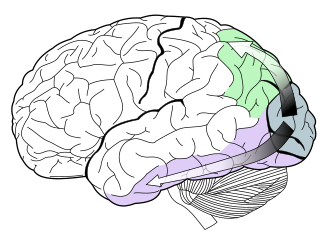
\includegraphics[width=0.6\textwidth]{../images/brain.png}
        \caption{Figur 1: caption. }
    \end{figure})

    noteringar:


    Arbetsminnet är en process i hjärnan där den medvetet plockar fram och manipulerar relevanta information.
    Det handlar om olika scenarion som stimulerar hjärnan och får den att selektivt välja minnen som passar in.
    Det är inte ofta nämnt att minnet som lagras är begränsat och temporär som den är.
    Med konstant upprepning och repetition så kan du manipulera minnet så att de sitter bättre.

    Men genom musiken ska minnet få fram en ett mer stabilt och sekvent arbete,utan att fokuset bryts av oljud.
    På så sätt få en mentalt lugnare miljö  för att lagra det visuella och informativa.

    BILD

    \begin{itemize} Hjärnan har flertal regioner inom sig där olika minnen lagras. Figur 1 visar de olika regionerna \end{itemize}

    Känner du igen en fråga på ett prov så får hjärnan signalera om tidigare aktivitet. \end{itemize}
    \begin{itemize} Informationen är lagrad i arbetsminnet under en kort period tills repetition uppstår. \end{itemize}


    \subsection{Visuella memory}
    Visuella memory är förmågan där minnet kopplas till vad synen tar upp.
    Det information som synen tar in skickas vidare till hjärnan.
    Specifikt så hamnar de i Posterior parietal cortex, vilket är en av de fyra stora delarna i hjärnan för att den ska fungera.
    Posterior parietal cortex uppfattas som funktionen för uppmärksammhet, arbetsminne och det visuella bilderna som ligger i minnet.
    Det är också det som gör så att vi kan planera vad nästa steg ska vara och kontrollera.
    \textcite{Capacitylimit}


    \subsection{Manipulering av information}
    Definitionen av att manipulera information är att kunna styra och kontrollera det.
    Det finns flertal sätt att manipuleras minnet.
    Att komma ihåg något under en längre tid är en process där du konstant repeterar information så att fastnar längre.




    \subsection{Liknande studie}




    \section{Metod}
    I denna undersökning så kommer en grupp av personer bli indelad i två olika testgrupper: A och B, för att avgöra om musik faktist förbättrar arbetsminnet.
    Genre på musik är en stor faktor gällande arbetsminne, så Grupp A får hörlurar där klassiskt musik spelas och grupp B gör undersökningen ljudlöst.
    \newline För att avgöra detta så används memory spel som ett verktyg.
    I detta fall så ska memory spelet visa 30 styckna kort med olika bilder på, korten visas i 30 sekunder innan dem vänds.
    \newline Alla kort ligger på samma ställe för alla, för att det ska vara rättvist och minska slumpäss faktorn.
    Målet är att komma ihåg så många kort som möjligt och med hjälp av musiken länka det visuella till ljud.
    Arbetet utförs enskilt för att mäta hur mycket varje individ kommer ihåg utan någon påverkan av andra.

    \subsection{Memory spel}
    Spelet ska kodas från grund med hjälp av visual studio code.
    Sidan är uppbygd av css kod vilket betyder att det finns en index.
    En Index fil fungerar som hemsida för webben.
    I den så importeras bilderna som ska vara på korten från assets mappen.
    För att korten ska fungera så finns det en javascript för Index filen.
    Vilket innehåller slumpässfaktorn för kortens positioner och vad som ska hända när man väljer olika kort.
    Att dem ska vända sig och om svaret är rätt eller fel.


    FORTS.
    Först ska sidan visa två alternativ, Grupp A eller grupp B.

    Sidan ska laddas upp på Glitch därefter.
    Glitch är en webbsida som tar in data.
    Så från testsidan så skickas svaren in till Glitch och all information samlas på samma ställe.
    Detta underlättar mätningen av resultaten i slutändan.

    Länk till projektet: https://endaxe.github.io/te-21-canvas/


    \subsection{Process}
    Testet inleds med att presentera kort för deltagarna vad arbetet handlar om.
    Presentationen ska klargöra varför detta utförs och vad målet med undersökningen är.
    Sedan blir deltagarna indelade i två grupper, A och B för att därefter få materialen som krävs för respektiv grupp, hörlurar för de i grupp A.
    Innan testet faktist börjar och för att det ska bli så riskfritt så möjligt så kommer instruktionerna precis innan.
    Det innehåller spelets innehåll, regler och vad målet är med det.
    Länken för memory spelet delas ut i ett classroom där all deltagande har tillgång till.
    Väl inne i memory spelet så kommer två alternativ att visa sig: alternativ A och alternativ B.
    Detta existerar för att dela in svaren som kommer in.
    Grupp A ska välja alternativet A och grupp B ska välja B.
    \newline Efter så sätts hörlurarna på för de som har det.
    Under en begränsad tid på max 10 minuter så bör alla ha startat spelet.
    Det är 30 kort totalt och med hälp av att korten visar sig 30 sekunder i början av spelets gång, så ska deltagarna para ihop så många par så möjligt med så lite fel så möjligt innan tiden tar slut.
    Då spelets gång är klar oavsett om det är för att tiden tog slut eller att man parat alla så avslutas det.
    När alla som har deltagit är klara så skickas all resultat och data till Glitch.
    Vilket gör att det sedan kan göras en beräkning av en slutsats om vilken grupp som presterat bättre än den andra.



    \subsection{Urval}
    Selektionen av detta arbete består av medelstora klasser på gymnasie nivå.
    Deltagande elever kommer att vara i åldrarna mellan 16 till 18 år.
    Detta är relevant efersom åldersgruppen i gymnasieskolor använder mycket digital läromedel vilket påverkar koncentrationsförmågan på olika sätt.
    Flertal skolor är osäkra om det faktist hjälper eleverna eller om det bara är en annan störningsmoment.
    Åldrarna i gymnasiet är målgruppen där detta är som mest relevant.
    Detta skapar ett tillfälle för en studie som kan säga på ett ungefär om läromedlet är positiv för inlärningen.


    \subsection{Etik}
    Valet att delta är helt valfritt och de som inte vill vara med behöver inte det.
    Datan som samlas in är helt anonymt och visar ingen uppgiven namn.
    Resultaten består endast av siffror, procent och om test-personen var i grupp A eller grupp B.
    Det enda undantaget är test klassen namn, vilket krävs för att kunna identifera och gruppera varsifrån data samlats in ifrån.


    \subsection{Analys av data}
    Görs efter datainsamling:
    Jämförelser mellan grupperna, vad är de som jämförs?
    Det kommer att vara 15 par där du får rätt genom att först klicka på ett kort och därefter hitta den andra direkt efter.
    Blir det fel så räknas det som 1 fel.
    Max 15 rätt men antalet fel kommer att varieras
    Student’s t-test

    \begin{figure}
        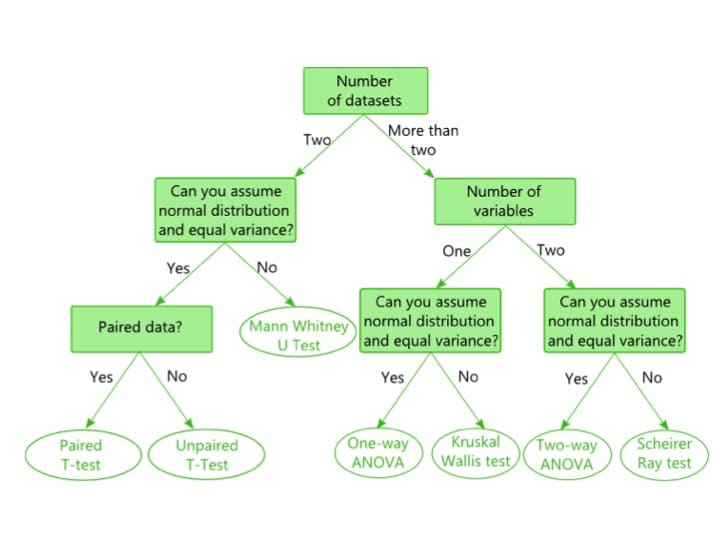
\includegraphics[width=0.8\textwidth]{../images/data.jpg}
        \caption{Figur 1: caption. }
    \end{figure})

    https://bitesizebio.com/19298/comparing-two-sets-of-data/


    \subsection{Diskussion}
    Det har många faktorer som kan anting försämra eller förbättra detta, som vilken genre musiken är eller personens koncentrationsnivå ligger på.

    Spelen som redan existerade på nätet var för slumpässiga för att få ett rättvist och en stabil resultat.
    det fel som inte var passande för undersökningen: korten blandades om för varje omgång som spelades och visades inte i början, vilket gör att de första kortvändingarna ökar felmarginalen.
    Så för att undvika detta så ska

    \printbibliography

\end{document}
